\documentclass[aspectratio=169,10pt]{beamer}
% =====================================================================
%  Le Collé — thème de présentation (même palette et mêmes notations que la fiche)
% =====================================================================
\usepackage[utf8]{inputenc}
\usepackage[T1]{fontenc}
\usepackage[sc]{mathpazo}
\usepackage[scaled=0.92]{helvet}
\usefonttheme{professionalfonts}
\usepackage{amsmath,amssymb,mathrsfs,stmaryrd}
\usepackage{microtype}
\usepackage{booktabs,array,multicol}
\usepackage[most]{tcolorbox}
\usepackage{tikz,pgfplots}
\usetikzlibrary{arrows.meta,calc,positioning,decorations.pathreplacing,shapes.misc}
\pgfplotsset{compat=1.17,trig format plots=rad}
\usepackage{tkz-tab}

% ---------- palette (identique à la fiche) ----------
\definecolor{Ink}{HTML}{1C2533}\definecolor{Bleu}{HTML}{1F3A5F}\definecolor{BleuMoyen}{HTML}{4A6A8F}
\definecolor{BleuClair}{HTML}{9DB2C9}\definecolor{Fond}{HTML}{F2F4F7}\definecolor{Ocre}{HTML}{B07A26}
\definecolor{Brique}{HTML}{A23B2A}\definecolor{Gris}{HTML}{5E6672}\definecolor{Filet}{HTML}{C5CCD6}
\definecolor{Vert}{HTML}{2E6B4F}

% ---------- notations (identiques à la fiche) ----------
\newcommand{\K}{\mathbb{K}}\newcommand{\R}{\mathbb{R}}\newcommand{\C}{\mathbb{C}}\newcommand{\Z}{\mathbb{Z}}
\newcommand{\Mn}[1]{\mathcal{M}_{n}(#1)}\newcommand{\rg}{\operatorname{rg}}\newcommand{\vect}{\operatorname{Vect}}
\newcommand{\Mat}{\operatorname{Mat}}\newcommand{\Id}{\operatorname{Id}}\newcommand{\com}{\operatorname{com}}
\newcommand{\vv}[1]{\overrightarrow{#1}}\newcommand{\ve}[1]{\vec{#1}}
\newcommand{\dt}[1]{\left|\begin{matrix}#1\end{matrix}\right|}
\DeclareRobustCommand{\HP}{{\sffamily\bfseries\scriptsize\textcolor{Brique}{[HP]}}}

% ---------- réglages beamer ----------
\setbeamertemplate{navigation symbols}{}
\setbeamersize{text margin left=0.85cm,text margin right=0.85cm}
\setbeamercolor{normal text}{fg=Ink,bg=white}
\setbeamercolor{structure}{fg=Bleu}
\setbeamercolor{alerted text}{fg=Brique}
\setbeamerfont{alerted text}{series=\bfseries}
\setbeamertemplate{itemize item}{\raisebox{0.15em}{\textcolor{Ocre}{\rule{0.38em}{0.38em}}}}
\setbeamertemplate{itemize subitem}{\textcolor{BleuMoyen}{\scriptsize\textbullet}}
\setbeamertemplate{enumerate item}{\textcolor{Bleu}{\sffamily\bfseries\insertenumlabel.}}
\setlength{\leftmargini}{1.2em}
\setbeamertemplate{blocks}[default]

% numéro de la partie courante, rappelé dans le titre et le pied de page (renvoi à la fiche)
\def\fichesec{}\def\chapnom{}
\newcommand{\chapitre}[1]{\def\chapnom{#1}}

\setbeamertemplate{frametitle}{%
  \vskip0.28cm
  \ifx\fichesec\empty\else
    \tikz[baseline=(b.base)]\node[fill=Ocre,text=white,font=\sffamily\bfseries\scriptsize,inner sep=2.5pt,rounded corners=1pt](b){\fichesec};\hspace{0.45em}%
  \fi
  {\color{Bleu}\sffamily\bfseries\Large\insertframetitle}\par
  \vskip0.06cm{\color{Filet}\rule{\linewidth}{0.5pt}}\vskip-0.2cm}

\setbeamertemplate{footline}{%
  \hbox to\paperwidth{%
    \hspace*{0.85cm}{\scriptsize\sffamily\color{Gris}Le Collé\ \ \textcolor{Filet}{|}\ \ \chapnom}\hfill
    {\scriptsize\sffamily\color{Gris}\ifx\fichesec\empty\else fiche \textbf{\color{Ocre}§\fichesec}\quad\fi\insertframenumber}\hspace*{0.85cm}}%
  \vskip0.18cm
  \hbox{\begin{tikzpicture}
    \fill[Fond] (0,0) rectangle (\paperwidth,2.2pt);
    \pgfmathsetmacro\prog{min(\insertframenumber/max(\inserttotalframenumber,1),1)}
    \fill[Ocre] (0,0) rectangle ({\prog*\paperwidth},2.2pt);
  \end{tikzpicture}}}

% ---------- encadrés : même code couleur que la fiche ----------
\tcbset{sb/.style={enhanced,arc=1pt,boxrule=0pt,left=6pt,right=6pt,top=3pt,bottom=3pt,before skip=0.14cm,after skip=0.14cm,
  fontupper=\normalsize\raggedright}}
\newcommand{\etiq}[2]{{\sffamily\bfseries\scriptsize\color{#1}\MakeUppercase{#2}}\par\vspace{2pt}}
\newtcolorbox{DEF}[1][Définition]{sb,colback=white,borderline west={2pt}{0pt}{Bleu},before upper={\etiq{Bleu}{#1}}}
\newtcolorbox{PROP}[1][Propriété]{sb,colback=Fond,borderline west={3pt}{0pt}{Bleu},before upper={\etiq{Bleu}{#1}}}
\newtcolorbox{FORM}[1][Formule]{sb,colback=white,colframe=BleuMoyen,boxrule=0.6pt,before upper={\etiq{BleuMoyen}{#1}}}
\newtcolorbox{METH}[1]{sb,colback=white,borderline north={1pt}{0pt}{Bleu},borderline south={1pt}{0pt}{Bleu},
  before upper={{\sffamily\bfseries\scriptsize\colorbox{Bleu}{\color{white}MÉTHODE}\ \color{Bleu}#1}\par\vspace{3pt}}}
\newtcolorbox{PIEGE}[1][Piège]{sb,colback=Brique!6,borderline west={2pt}{0pt}{Brique},before upper={\etiq{Brique}{#1}}}
\newtcolorbox{ASTU}[1][Astuce]{sb,colback=Ocre!8,borderline west={2pt}{0pt}{Ocre},before upper={\etiq{Ocre}{#1}}}
\newtcolorbox{HPBOX}{sb,colback=white,borderline west={2pt}{0pt}{Brique},before upper={\etiq{Brique}{Hors programme}}}
\newtcolorbox{ATOI}[1][À toi]{sb,colback=Vert!6,borderline west={2pt}{0pt}{Vert},before upper={\etiq{Vert}{#1}}}
\newtcolorbox{RETENIR}{sb,colback=Bleu!5,colframe=Bleu,boxrule=0.8pt,left=8pt,
  before upper={\etiq{Bleu}{À retenir}}}
\newtcolorbox{EX}[1][Exemple]{sb,colback=white,colframe=Filet,boxrule=0.5pt,before upper={\etiq{Gris}{#1}}}

% complément pédagogique absent du livre : étiquette pointillée
\DeclareRobustCommand{\ajout}{\tikz[baseline=(a.base)]\node[draw=Gris,dashed,text=Gris,font=\sffamily\scriptsize,inner sep=2pt,rounded corners=1pt](a){complément hors livre};}
\DeclareRobustCommand{\livre}[1]{{\sffamily\scriptsize\color{Gris}[livre #1]}}
\newcommand{\rep}[1]{\textcolor{Vert}{#1}}% réponse attendue de l'élève

% ---------- styles de figures (identiques au livre) ----------
\pgfplotsset{courbe/.style={axis lines=middle,axis equal image,
  axis line style={Gris,-{Stealth[length=4pt]}},
  xlabel={$x$},ylabel={$y$},ticklabel style={font=\scriptsize\sffamily,color=Gris},
  every axis x label/.style={at={(ticklabel* cs:1)},anchor=west,font=\small},
  every axis y label/.style={at={(ticklabel* cs:1)},anchor=south,font=\small},
  samples=200,smooth}}
\pgfplotsset{mini/.style={axis lines=middle,axis line style={Filet},xtick=\empty,ytick=\empty,width=3.9cm,height=3.9cm,
  xmin=-1.15,xmax=1.15,ymin=-1.15,ymax=1.15,title style={font=\footnotesize\sffamily,yshift=-0.1cm},samples=100}}
\tikzset{arcetude/.style={Bleu,line width=1.25pt},
         reste/.style={BleuClair,line width=1pt},
         tgte/.style={Ocre,line width=1pt},
         asy/.style={Gris,dashed,line width=0.7pt},
         pt/.style={circle,fill=Ink,inner sep=1.3pt},
         >={Stealth[length=5pt]}}

% ---------- diapositives de partie ----------
% \partie{num}{titre}{question guide}{liste des parties du chapitre via \rm}
\newcommand{\rmitem}[2]{\def\tmp{#1}%
  \ifx\tmp\fichesec{\color{Bleu}\bfseries #1\quad #2}\else{\color{Gris!70}#1\quad #2}\fi\par\vspace{2pt}}
\newcommand{\partie}[4]{%
  \def\fichesec{#1}\section{#2}%
  \begin{frame}[plain]
  \begin{tikzpicture}[remember picture,overlay]
    \fill[Bleu] (current page.north west) rectangle ([xshift=6.3cm]current page.south west);
    \node[anchor=north west,text=white,font=\sffamily\bfseries\fontsize{40}{40}\selectfont] at ([xshift=0.8cm,yshift=-1.2cm]current page.north west) {#1};
    \node[anchor=north west,text width=4.8cm,align=left,text=white,font=\sffamily\bfseries\Large] at ([xshift=0.8cm,yshift=-2.9cm]current page.north west) {\hyphenpenalty=10000\exhyphenpenalty=10000 #2\par};
    \node[anchor=south west,text width=4.8cm,text=white!75!Bleu,font=\sffamily\scriptsize] at ([xshift=0.8cm,yshift=0.6cm]current page.south west) {\chapnom\\fiche \textbf{§#1}};
  \end{tikzpicture}
  \hspace*{5.5cm}\begin{minipage}{8.4cm}
  {\sffamily\scriptsize\color{Ocre}\bfseries LA QUESTION}\par\vspace{2pt}
  {\large #3}\par\vspace{0.7cm}
  {\sffamily\scriptsize\color{Gris}\bfseries DANS CE CHAPITRE}\par\vspace{4pt}
  {\sffamily\small #4}
  \end{minipage}
  \end{frame}}



% ---------- exercices en séance : énoncé sur une diapositive, correction sur la suivante ----------
\newcommand{\badgeexo}[1]{\tikz[baseline=(e.base)]\node[fill=Vert,text=white,font=\sffamily\bfseries\scriptsize,inner sep=2.5pt,rounded corners=1pt](e){EXERCICE #1};\hspace{0.4em}}
\newcommand{\badgecor}[1]{\tikz[baseline=(e.base)]\node[draw=Vert,line width=0.8pt,text=Vert,font=\sffamily\bfseries\scriptsize,inner sep=2.2pt,rounded corners=1pt](e){CORRECTION #1};\hspace{0.4em}}
\newtcolorbox{ENONCE}[1][]{sb,colback=Vert!6,borderline west={3pt}{0pt}{Vert},left=9pt,top=5pt,bottom=5pt,
  before upper={{\sffamily\bfseries\scriptsize\color{Vert}À TOI\ifx\relax#1\relax\else\ \ ·\ \ \MakeUppercase{#1}\fi}\par\vspace{4pt}}}
\newtcolorbox{INDICE}{sb,colback=white,colframe=Vert!60,boxrule=0.5pt,borderline={0.5pt}{0pt}{Vert!60,dashed},
  before upper={\etiq{Vert}{Indice (si besoin)}}}
\newtcolorbox{RAIS}[1][Le raisonnement]{sb,colback=Vert!5,borderline west={2pt}{0pt}{Vert},before upper={\etiq{Vert}{#1}}}
\newtcolorbox{OUTIL}{sb,colback=Fond,borderline west={2pt}{0pt}{Bleu},before upper={\etiq{Bleu}{Propriété ou méthode utilisée}}}
\newcommand{\etape}[1]{{\sffamily\bfseries\footnotesize\color{Vert}#1}\ }
\newcommand{\objectif}[1]{\par\vspace{2pt}{\footnotesize\sffamily\color{Gris}Objectif : #1}}
\newcommand{\Ker}{\operatorname{Ker}}\renewcommand{\Im}{\operatorname{Im}}\newcommand{\tr}{\operatorname{tr}}\newcommand{\Sp}{\operatorname{Sp}}
\newcommand{\GLn}[1]{\mathrm{GL}_n(#1)}
\title{Le Collé --- Séries numériques}

\begin{document}

% ---------------------------------------------------------------- titre
\begin{frame}[plain]
\begin{tikzpicture}[remember picture,overlay]
  \fill[Bleu] (current page.north west) rectangle (current page.south east);
  \node[anchor=north west,text=white!70!Bleu,font=\sffamily\scriptsize] at ([xshift=1cm,yshift=-1.2cm]current page.north west)
    {LE COLLÉ\ \ ·\ \ MATHÉMATIQUES PT\ \ ·\ \ CHAPITRE 7\ \ ·\ \ SUPPORT DE SÉANCE};
  \node[anchor=north west,text=white,font=\sffamily\bfseries\fontsize{26}{30}\selectfont,text width=13cm] at ([xshift=1cm,yshift=-2.1cm]current page.north west)
    {Séries numériques};
  \fill[Ocre] ([xshift=1cm,yshift=-4.6cm]current page.north west) rectangle ([xshift=4cm,yshift=-4.65cm]current page.north west);
  \node[anchor=north west,text=white!80!Bleu,font=\normalsize,text width=12.5cm] at ([xshift=1cm,yshift=-5cm]current page.north west)
    {Présentation pour expliquer, avec cinq exercices à chercher en séance ;\\ le \textbf{livret} pour relire, la \textbf{fiche} pour réviser.
     Mêmes parties (§1.1 à §1.6), mêmes notations.};
\end{tikzpicture}
\end{frame}

% ---------------------------------------------------------------- plan
\begin{frame}{Plan : trois séances de 2 h}
\begin{columns}[T]
\column{0.56\textwidth}
\small
\renewcommand{\arraystretch}{1.3}
\begin{tabular}{@{}l l r@{}}
\multicolumn{3}{@{}l}{\sffamily\bfseries\color{Ocre}Séance 1 --- outils et définitions}\\
\textbf{\color{Bleu}1.1} & Rappels sur les suites & \color{Vert}Ex.~1\\
\textbf{\color{Bleu}1.2} & Séries : définitions, exemples & \color{Vert}Ex.~2\\[2pt]
\multicolumn{3}{@{}l}{\sffamily\bfseries\color{Ocre}Séance 2 --- termes positifs}\\
\textbf{\color{Bleu}1.3} & Comparaison, Riemann, d'Alembert & \color{Vert}Ex.~3\\[2pt]
\multicolumn{3}{@{}l}{\sffamily\bfseries\color{Ocre}Séance 3 --- signe quelconque}\\
\textbf{\color{Bleu}1.4} & Convergence absolue, alternées & \color{Vert}Ex.~4\\
\textbf{\color{Bleu}1.5} & Produit de Cauchy & \\
\textbf{\color{Bleu}1.6} & Synthèse & \color{Vert}Ex.~5
\end{tabular}
\column{0.4\textwidth}
\begin{ASTU}[Le fil du chapitre]
\small Une question : \textbf{la somme infinie $u_0+u_1+\cdots$ a-t-elle un sens ?}\\[3pt]
On le décide le plus souvent \textbf{sans calculer} la somme, en comparant à des séries de référence.
\end{ASTU}
{\small\color{Gris}Prérequis : suites (PTSI), développements limités, intégrales sur un segment.}
\end{columns}
\end{frame}

\chapitre{Chapitre 7 · Séries numériques}
\newcommand{\rmI}{\rmitem{1.1}{Rappels sur les suites}\rmitem{1.2}{Séries : définitions}\rmitem{1.3}{Termes positifs}
  \rmitem{1.4}{Convergence absolue, alternées}\rmitem{1.5}{Produit de Cauchy}\rmitem{1.6}{Synthèse}}

\begin{frame}{Le problème : additionner une infinité de nombres}
\begin{columns}[T]
\column{0.5\textwidth}
$1+\frac12+\frac14+\frac18+\cdots$ ?\quad On regarde les sommes \textbf{finies} :
\[S_n=1+\frac12+\dots+\frac1{2^n}=2-\frac1{2^n}\ \longrightarrow\ 2.\]
\pause
$1+\frac12+\frac13+\frac14+\cdots$ : les termes tendent vers $0$\dots\ mais $S_n\to+\infty$.\\[4pt]
\pause
$1-1+1-1+\cdots$ : $S_n$ vaut $1,0,1,0,\dots$ : pas de limite.
\column{0.46\textwidth}
\centering
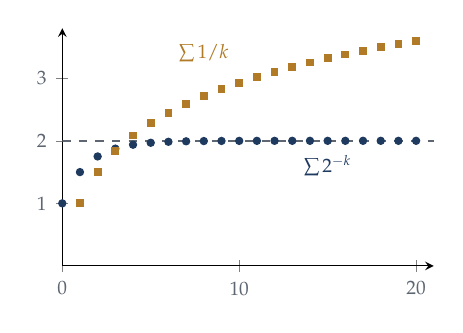
\begin{tikzpicture}
\begin{axis}[width=6.3cm,height=4.6cm,axis lines=left,xmin=0,xmax=21,ymin=0,ymax=3.8,
  ticklabel style={font=\scriptsize\sffamily,color=Gris},xtick={0,10,20},ytick={1,2,3}]
\addplot[only marks,mark=*,mark size=1.3pt,Bleu,samples at={0,...,20}] {2-2^(-x)};
\addplot[only marks,mark=square*,mark size=1.2pt,Ocre] coordinates {(1,1)(2,1.5)(3,1.8333)(4,2.0833)(5,2.2833)(6,2.45)(7,2.5929)(8,2.7179)(9,2.829)(10,2.929)(11,3.0199)(12,3.1032)(13,3.1801)(14,3.2516)(15,3.3182)(16,3.3807)(17,3.4396)(18,3.4951)(19,3.5477)(20,3.5977)};
\addplot[asy,domain=0:21] {2};
\node[font=\scriptsize\sffamily,Bleu] at (axis cs:15,1.6) {$\sum 2^{-k}$};
\node[font=\scriptsize\sffamily,Ocre] at (axis cs:8,3.4) {$\sum 1/k$};
\end{axis}
\end{tikzpicture}
\end{columns}
\pause
\begin{RETENIR}
La somme d'une série est la \textbf{limite} de ses sommes partielles, quand elle existe. Le chapitre donne les outils pour
\textbf{décider} si elle existe.
\end{RETENIR}
\end{frame}

% =====================================================================
\partie{1.1}{Rappels sur les suites}{Quels outils sur les suites servent à chaque ligne ?}{\rmI}

\begin{frame}{Trois théorèmes d'existence (suites réelles)}
\begin{PROP}[Limite monotone \livre{th.~1.4}]
Croissante et majorée $\Rightarrow$ converge ; croissante non majorée $\Rightarrow\ \to+\infty$.
\end{PROP}
\pause
\begin{PROP}[Suites adjacentes \livre{th.~1.5}]
$(a_n)\nearrow$, $(b_n)\searrow$, $b_n-a_n\to0$ $\Rightarrow$ même limite $\ell$, et $a_n\leq\ell\leq b_n$.
\end{PROP}
\pause
\begin{columns}[T]
\column{0.48\textwidth}
\begin{PROP}[Gendarmes]
$u_n\leq v_n\leq w_n$, $u_n,w_n\to\ell$ $\Rightarrow v_n\to\ell$.
\end{PROP}
\column{0.48\textwidth}
\begin{ASTU}[Pourquoi ici ?]
Limite monotone $\to$ séries à termes positifs ; adjacentes $\to$ séries alternées.
\end{ASTU}
\end{columns}
\end{frame}

\begin{frame}{Comparer des suites : $\sim$, $o$, $O$}
\begin{DEF}[Définition]
$u_n\sim v_n$ si $\frac{u_n}{v_n}\to1$ ;\quad $u_n=o(v_n)$ si $\frac{u_n}{v_n}\to0$ ;\quad $u_n=O(v_n)$ si $\frac{u_n}{v_n}$ est bornée.
\end{DEF}
\pause
\begin{columns}[T]
\column{0.5\textwidth}
\begin{PROP}[Règles]
$u_n\sim v_n\iff u_n=v_n+o(v_n)$ ; même signe à partir d'un rang ; produits, quotients, puissances fixes.
\end{PROP}
\column{0.46\textwidth}
\begin{PIEGE}
On n'\textbf{additionne} pas, on ne \textbf{compose} pas les équivalents : $n+1\sim n$ mais $e^{n+1}\not\sim e^n$.
\end{PIEGE}
\end{columns}
\pause
\begin{FORM}[Croissances comparées]
$(\ln n)^\alpha=o(n^\beta)$,\quad $n^\alpha=o(a^n)$ ($a>1$),\quad $a^n=o(n!)$,\quad $n!=o(n^n)$.
\end{FORM}
\end{frame}

\begin{frame}{Développements limités : l'outil principal}
\small
\begin{columns}[T]
\column{0.5\textwidth}
\begin{FORM}[En $0$]
$e^x=1+x+\frac{x^2}2+o(x^2)$\\
$\ln(1+x)=x-\frac{x^2}2+\frac{x^3}3+o(x^3)$\\
$\cos x=1-\frac{x^2}2+o(x^3)$,\ $\sin x=x-\frac{x^3}6+o(x^4)$\\
$(1+x)^\alpha=1+\alpha x+\frac{\alpha(\alpha-1)}2x^2+o(x^2)$
\end{FORM}
\column{0.46\textwidth}
\begin{METH}{Trouver un équivalent \livre{méth.~1.1}}
1. Factoriser le terme dominant.\\
2. $a_n^{b_n}=\exp(b_n\ln a_n)$.\\
3. Développer jusqu'au premier terme non nul.
\end{METH}
\end{columns}
\pause
\begin{EX}
$\left(1+\frac1n\right)^n=\exp\!\big(n\ln(1+\tfrac1n)\big)=\exp\!\left(1-\frac1{2n}+o(\tfrac1n)\right)\to e$.
\end{EX}
\end{frame}

\begin{frame}{\badgeexo{1}Un équivalent}
\begin{ENONCE}[8 min]
Montrer que $\left(1+\frac1n\right)^n-e\sim-\frac e{2n}$.
\objectif{composer correctement par l'exponentielle.}
\end{ENONCE}
\pause
\begin{INDICE}
Écrire $\left(1+\frac1n\right)^n-e=e\left(e^{x_n-1}-1\right)$ avec $x_n=n\ln\left(1+\frac1n\right)$.
\end{INDICE}
\end{frame}

\begin{frame}{\badgecor{1}Un équivalent}
\begin{columns}[T]
\column{0.4\textwidth}
\begin{RAIS}
On ne compose pas les équivalents par $\exp$ : on isole $e^{y}-1$ avec $y\to0$, qui, lui, est équivalent à $y$.
\end{RAIS}
\column{0.57\textwidth}
\etape{1.} $x_n=n\left(\frac1n-\frac1{2n^2}+o(\frac1{n^2})\right)=1-\frac1{2n}+o(\frac1n)$.\\[3pt]
\pause
\etape{2.} $\left(1+\frac1n\right)^n-e=e\left(e^{x_n-1}-1\right)$, et $x_n-1\to0$.\\[3pt]
\pause
\etape{3.} $e^y-1\sim y$ : $\left(1+\frac1n\right)^n-e\sim e(x_n-1)\sim-\frac e{2n}$.
\end{columns}
\end{frame}

% =====================================================================
\partie{1.2}{Séries : définitions, premiers exemples}{Que veut dire « la série converge » ?}{\rmI}

\begin{frame}{Série, somme partielle, somme, reste}
\begin{DEF}[Définition \livre{déf.~1.10}]
$S_n=\sum_{k=0}^nu_k$. La \emph{série} $\sum u_n$ est la suite $(S_n)$. Elle \emph{converge} si $(S_n)$ converge ;
sa limite est la \emph{somme} $\sum_{n=0}^{+\infty}u_n$. Le \emph{reste} est $R_n=\sum_{k=n+1}^{+\infty}u_k$.
\end{DEF}
\pause
\begin{columns}[T]
\column{0.5\textwidth}
\begin{PROP}[Linéarité, reste \livre{prop.~1.11}]
Somme de deux séries convergentes : convergente. $R_n\to0$. Convergente $+$ divergente : divergente.
\end{PROP}
\column{0.46\textwidth}
\begin{PIEGE}
N'écrire $\sum_{n=0}^{+\infty}u_n$ (un nombre) \textbf{qu'après} avoir prouvé la convergence.
\end{PIEGE}
\end{columns}
\end{frame}

\begin{frame}{Une condition nécessaire : $u_n\to0$}
\begin{PROP}[Divergence grossière \livre{th.~1.12}]
Si $\sum u_n$ converge, alors $u_n\to0$. \quad Démonstration : $u_n=S_n-S_{n-1}\to S-S=0$.
\end{PROP}
\pause
\begin{columns}[T]
\column{0.48\textwidth}
\begin{EX}
$\sum1$, $\sum(-1)^n$, $\sum\cos n$, $\sum\left(1+\frac1n\right)^n$ : divergence grossière.
\end{EX}
\column{0.48\textwidth}
\begin{PIEGE}
La réciproque est \textbf{fausse} : $\frac1n\to0$, mais $\sum\frac1n$ diverge.
\end{PIEGE}
\end{columns}
\pause
\begin{RETENIR}
« $u_n\to0$ ? » est le \textbf{premier test}. Il peut prouver la divergence, jamais la convergence.
\end{RETENIR}
\end{frame}

\begin{frame}{Séries de référence}
\begin{columns}[T]
\column{0.5\textwidth}
\begin{PROP}[Télescopiques \livre{th.~1.14}]
$(a_n)$ converge $\iff\sum(a_{n+1}-a_n)$ converge, et $\sum_{n=0}^{+\infty}(a_{n+1}-a_n)=\lim a_n-a_0$.
\end{PROP}
\pause
\begin{EX}
$\frac1{n(n+1)}=\frac1n-\frac1{n+1}$ : $\sum_{k=1}^n=1-\frac1{n+1}\to1$.
\end{EX}
\column{0.46\textwidth}
\pause
\begin{PROP}[Géométriques \livre{th.~1.16}]
$\sum q^n$ converge $\iff|q|<1$ ; somme $\frac1{1-q}$.
\end{PROP}
\pause
\begin{PROP}[Exponentielle \livre{th.~1.17}]
$\sum\frac{x^n}{n!}=e^x$ pour tout $x\in\R$.
\end{PROP}
\end{columns}
\end{frame}

\begin{frame}{\badgeexo{2}Deux télescopages}
\begin{ENONCE}[10 min]
\begin{enumerate}
\item Calculer $\sum_{n=1}^{+\infty}\frac1{n(n+1)(n+2)}$.
\item Montrer que $\sum_{n\geq2}\ln\left(1-\frac1{n^2}\right)$ converge et calculer sa somme.
\end{enumerate}
\objectif{faire apparaître une différence $a_n-a_{n+1}$.}
\end{ENONCE}
\pause
\begin{INDICE}
(1) $\frac1{n(n+1)(n+2)}=\frac12\left(\frac1{n(n+1)}-\frac1{(n+1)(n+2)}\right)$.\quad (2) $1-\frac1{n^2}=\frac{(n-1)(n+1)}{n^2}$.
\end{INDICE}
\end{frame}

\begin{frame}{\badgecor{2}Deux télescopages}
\begin{columns}[T]
\column{0.38\textwidth}
\begin{RAIS}
On ne cherche pas à « sommer » : on écrit le terme comme une différence, et presque tout se simplifie.
\end{RAIS}
\column{0.59\textwidth}
\etape{1.} Avec $a_n=\frac1{2n(n+1)}$ : terme $=a_n-a_{n+1}$, donc la somme vaut $a_1-\lim a_n=\frac14$.\\[4pt]
\pause
\etape{2.} $\ln\left(1-\frac1{k^2}\right)=\big(\ln(k+1)-\ln k\big)-\big(\ln k-\ln(k-1)\big)$.\\
$\sum_{k=2}^n=\ln\frac{n+1}n-\ln2\to-\ln2$.
\end{columns}
\end{frame}

% =====================================================================
\partie{1.3}{Séries à termes positifs}{Comment décider sans calculer la somme ?}{\rmI}

\begin{frame}{Le principe : des sommes partielles croissantes}
\begin{PROP}[\livre{th.~1.18}]
Si $u_n\geq0$, $(S_n)$ est croissante : $\sum u_n$ converge $\iff(S_n)$ est \textbf{majorée}. Sinon $S_n\to+\infty$.
\end{PROP}
\pause
\begin{columns}[T]
\column{0.5\textwidth}
\begin{PROP}[Comparaison \livre{th.~1.19}]
$0\leq u_n\leq v_n$ : $\sum v_n$ CV $\Rightarrow\sum u_n$ CV ;\ $\sum u_n$ DV $\Rightarrow\sum v_n$ DV.
\end{PROP}
\column{0.46\textwidth}
\pause
\begin{PROP}[Équivalents \livre{th.~1.20}]
$u_n\sim v_n$, \textbf{$v_n\geq0$} : même nature.
\end{PROP}
\end{columns}
\pause
\begin{PIEGE}
Sans hypothèse de signe, c'est faux : $\frac{(-1)^n}{\sqrt n}+\frac1n\sim\frac{(-1)^n}{\sqrt n}$, mais l'une diverge, l'autre converge.
\end{PIEGE}
\end{frame}

\begin{frame}{Comparer une série à une intégrale}
\begin{columns}[T]
\column{0.5\textwidth}
\centering
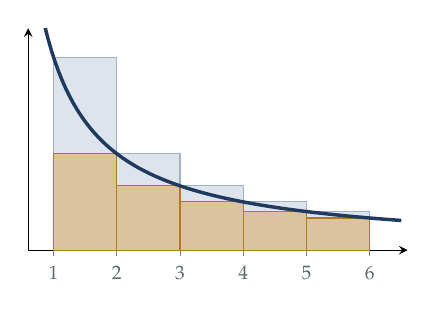
\begin{tikzpicture}
\begin{axis}[width=6.4cm,height=4.4cm,axis lines=left,xmin=0.6,xmax=6.6,ymin=0,ymax=1.15,
  ticklabel style={font=\scriptsize\sffamily,color=Gris},xtick={1,...,6},ytick=\empty]
\addplot[fill=BleuClair!35,draw=BleuClair] coordinates {(1,0) (1,1) (2,1) (2,0)} \closedcycle;
\addplot[fill=BleuClair!35,draw=BleuClair] coordinates {(2,0) (2,0.5) (3,0.5) (3,0)} \closedcycle;
\addplot[fill=BleuClair!35,draw=BleuClair] coordinates {(3,0) (3,0.3333) (4,0.3333) (4,0)} \closedcycle;
\addplot[fill=BleuClair!35,draw=BleuClair] coordinates {(4,0) (4,0.25) (5,0.25) (5,0)} \closedcycle;
\addplot[fill=BleuClair!35,draw=BleuClair] coordinates {(5,0) (5,0.2) (6,0.2) (6,0)} \closedcycle;
\addplot[fill=Ocre!45,draw=Ocre] coordinates {(1,0) (1,0.5) (2,0.5) (2,0)} \closedcycle;
\addplot[fill=Ocre!45,draw=Ocre] coordinates {(2,0) (2,0.3333) (3,0.3333) (3,0)} \closedcycle;
\addplot[fill=Ocre!45,draw=Ocre] coordinates {(3,0) (3,0.25) (4,0.25) (4,0)} \closedcycle;
\addplot[fill=Ocre!45,draw=Ocre] coordinates {(4,0) (4,0.2) (5,0.2) (5,0)} \closedcycle;
\addplot[fill=Ocre!45,draw=Ocre] coordinates {(5,0) (5,0.1667) (6,0.1667) (6,0)} \closedcycle;
\addplot[arcetude,domain=0.85:6.5,samples=100] {1/x};
\end{axis}
\end{tikzpicture}
\column{0.46\textwidth}
\begin{PROP}[\livre{th.~1.22}]
$f$ continue, positive, \textbf{décroissante} :
\[f(k+1)\leq\int_k^{k+1}f\leq f(k),\]
et $\sum f(n)$, $\int^{+\infty}f$ ont même nature.
\end{PROP}
\end{columns}
\pause
\begin{columns}[T]
\column{0.5\textwidth}
\begin{PROP}[Riemann \livre{th.~1.23}]
$\sum\frac1{n^\alpha}$ converge $\iff\alpha>1$.
\end{PROP}
\column{0.46\textwidth}
\begin{EX}
$\ln(n+1)\leq H_n\leq1+\ln n$, donc $H_n\sim\ln n$.
\end{EX}
\end{columns}
\end{frame}

\begin{frame}{La règle de d'Alembert}
\begin{PROP}[\livre{th.~1.25}]
$u_n>0$, $\frac{u_{n+1}}{u_n}\to\ell$ : si $\ell<1$, convergence ; si $\ell>1$, divergence grossière ; si $\ell=1$, \textbf{on ne sait pas}.
\end{PROP}
\pause
\begin{columns}[T]
\column{0.5\textwidth}
\begin{RAIS}[L'idée de la preuve]
Si $\ell<q<1$ : $u_{n+1}\leq qu_n$ à partir d'un rang, donc $u_n\leq Kq^n$ : comparaison à une série géométrique.
\end{RAIS}
\column{0.46\textwidth}
\begin{ASTU}[Quand l'utiliser]
Factorielles, $a^n$, $n^n$. Jamais pour une fraction rationnelle ($\ell=1$).
\end{ASTU}
\end{columns}
\pause
\begin{EX}
$\frac{n!}{n^n}$ : $\frac{u_{n+1}}{u_n}=\left(1+\frac1n\right)^{-n}\to\frac1e<1$ : convergente.
\end{EX}
\end{frame}

\begin{frame}{Méthode : série à termes positifs}
\begin{METH}{Quel outil ? \livre{méth.~1.3}}
\begin{enumerate}
\item Chercher un \textbf{équivalent} simple $v_n\geq0$.
\item Comparer à Riemann ou à une géométrique : $n^\alpha u_n\to0$ ($\alpha>1$) $\Rightarrow$ CV ; $nu_n\to+\infty\Rightarrow$ DV.
\item Factorielles, puissances $n$-ièmes : d'Alembert.
\item $u_n=f(n)$, $f$ décroissante, intégrale calculable : série-intégrale.
\end{enumerate}
\end{METH}
\pause
\begin{EX}
$\frac{\ln n}{n^2}=o\left(\frac1{n^{3/2}}\right)$ : CV.\quad $\frac1{\sqrt n\ln n}\geq\frac1n$ : DV.\quad $\frac1{n\ln n}$ : intégrale $\ln\ln X\to+\infty$, DV.
\end{EX}
\end{frame}

\begin{frame}{\badgeexo{3}Nature de séries à termes positifs}
\begin{ENONCE}[12 min]
Nature des séries de terme général :
\[\text{(a)}\ \frac{n^2+1}{n^4+3}\qquad\text{(b)}\ 1-\cos\frac1n\qquad\text{(c)}\ \frac1{\ln n+e^n}\qquad\text{(d)}\ n^2e^{-\sqrt n}\qquad\text{(e)}\ \frac{2^nn!}{n^n}.\]
\objectif{choisir le bon outil selon la forme du terme.}
\end{ENONCE}
\pause
\begin{INDICE}
(a)(b)(c) un équivalent. (d) montrer $n^4u_n\to0$. (e) d'Alembert.
\end{INDICE}
\end{frame}

\begin{frame}{\badgecor{3}Nature de séries à termes positifs}
\begin{columns}[T]
\column{0.36\textwidth}
\begin{RAIS}
Tous les termes sont positifs : on peut utiliser équivalents et comparaisons.
\end{RAIS}
\column{0.61\textwidth}
\etape{(a)} $\sim\frac1{n^2}$ : CV.\quad \etape{(b)} $\sim\frac1{2n^2}$ : CV.\\[3pt]
\pause
\etape{(c)} $\ln n=o(e^n)$, donc $\sim e^{-n}$ : CV (géométrique).\\[3pt]
\pause
\etape{(d)} $n^4u_n=e^{6\ln n-\sqrt n}\to0$ : $u_n=o(\frac1{n^2})$, CV.\\[3pt]
\pause
\etape{(e)} $\frac{u_{n+1}}{u_n}=2\left(1+\frac1n\right)^{-n}\to\frac2e<1$ : CV.
\end{columns}
\end{frame}

% =====================================================================
\partie{1.4}{Convergence absolue, séries alternées}{Et quand le signe change ?}{\rmI}

\begin{frame}{Convergence absolue}
\begin{DEF}[Définition \livre{déf.~1.28}]
$\sum u_n$ est \emph{absolument convergente} si $\sum|u_n|$ converge.
\end{DEF}
\pause
\begin{PROP}[\livre{th.~1.29 et 1.30}]
Absolument convergente $\Rightarrow$ convergente, et $\left|\sum u_n\right|\leq\sum|u_n|$.\\
Si $u_n=O(v_n)$ avec $\sum v_n$ convergente à termes positifs, $\sum u_n$ converge absolument.
\end{PROP}
\pause
\begin{columns}[T]
\column{0.5\textwidth}
\begin{RAIS}[L'idée de la preuve]
$u_n=u_n^+-u_n^-$ avec $0\leq u_n^\pm\leq|u_n|$ ; parties réelle et imaginaire pour $\C$.
\end{RAIS}
\column{0.46\textwidth}
\begin{EX}
$\frac{\cos n}{n^2}$, $\frac{e^{in\theta}}{n^{3/2}}$ : $|u_n|\leq\frac1{n^\alpha}$, $\alpha>1$.
\end{EX}
\end{columns}
\end{frame}

\begin{frame}{Le critère des séries alternées}
\begin{columns}[T]
\column{0.55\textwidth}
\begin{PROP}[\livre{th.~1.32}]
$(a_n)$ \textbf{positive, décroissante, de limite nulle} $\Rightarrow\sum(-1)^na_n$ converge, et $|R_n|\leq a_{n+1}$.
\end{PROP}
\pause
\begin{RAIS}[La preuve]
$(S_{2n})\searrow$, $(S_{2n+1})\nearrow$, $S_{2n+1}-S_{2n}=-a_{2n+1}\to0$ : suites adjacentes.
\end{RAIS}
\column{0.41\textwidth}
\centering
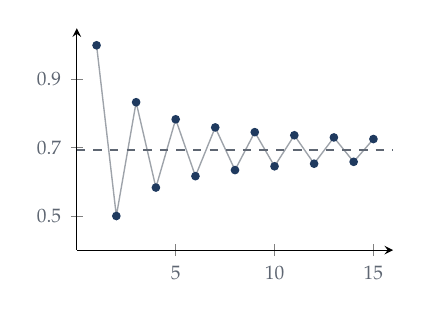
\begin{tikzpicture}
\begin{axis}[width=5.6cm,height=4.4cm,axis lines=left,xmin=0,xmax=16,ymin=0.4,ymax=1.05,
  ticklabel style={font=\scriptsize\sffamily,color=Gris},xtick={5,10,15},ytick={0.5,0.7,0.9}]
\addplot[Gris!60,line width=0.5pt,mark=*,mark size=1.3pt,mark options={fill=Bleu,draw=Bleu}] coordinates {(1,1)(2,0.5)(3,0.8333)(4,0.5833)(5,0.7833)(6,0.6167)(7,0.7595)(8,0.6345)(9,0.7456)(10,0.6456)(11,0.7365)(12,0.6532)(13,0.7301)(14,0.6587)(15,0.7254)};
\addplot[asy,domain=0:16] {0.6931};
\end{axis}
\end{tikzpicture}\\
{\scriptsize\color{Gris}$\sum\frac{(-1)^{k+1}}k$ : $S_n\to\ln2$}
\end{columns}
\pause
\begin{PIEGE}
Pour un signe variable : \textbf{pas d'équivalent}. $\frac{(-1)^n}{\sqrt n+(-1)^n}\sim\frac{(-1)^n}{\sqrt n}$, et pourtant la première série diverge.
\end{PIEGE}
\end{frame}

\begin{frame}{Méthode : développement asymptotique}
\begin{METH}{Signe quelconque \livre{méth.~1.4}}
Développer $u_n$ jusqu'à un reste $O\left(\frac1{n^\alpha}\right)$, $\alpha>1$ ; reconnaître chaque terme ; conclure par linéarité.
\end{METH}
\pause
\begin{EX}
$\frac{(-1)^n}{\sqrt n+(-1)^n}=\frac{(-1)^n}{\sqrt n}\cdot\frac1{1+\frac{(-1)^n}{\sqrt n}}
=\underbrace{\frac{(-1)^n}{\sqrt n}}_{\text{CV (critère)}}\ \underbrace{-\frac1n}_{\text{DV}}\ +\underbrace{O\left(\frac1{n^{3/2}}\right)}_{\text{CV abs.}}$
\quad : \textbf{divergente}.
\end{EX}
\end{frame}

\begin{frame}{\badgeexo{4}Séries de signe quelconque}
\begin{ENONCE}[12 min]
Nature des séries de terme général :
\[\text{(a)}\ \frac{(-1)^n}{n^\alpha}\ (\alpha\in\R)\qquad\text{(b)}\ \ln\left(1+\frac{(-1)^n}{\sqrt n}\right)\qquad\text{(c)}\ \frac{(-1)^n}{n+(-1)^n}.\]
\objectif{convergence absolue, critère, ou développement.}
\end{ENONCE}
\pause
\begin{INDICE}
(b) $\ln(1+x)=x-\frac{x^2}2+O(x^3)$. (c) Factoriser par $n$.
\end{INDICE}
\end{frame}

\begin{frame}{\badgecor{4}Séries de signe quelconque}
\begin{columns}[T]
\column{0.36\textwidth}
\begin{RAIS}
Absolue d'abord ; sinon le critère ; s'il ne s'applique pas, développer.
\end{RAIS}
\column{0.61\textwidth}
\etape{(a)} $\alpha\leq0$ : DV grossière ; $0<\alpha\leq1$ : CV (critère), pas absolue ; $\alpha>1$ : CV absolue.\\[3pt]
\pause
\etape{(b)} $u_n=\frac{(-1)^n}{\sqrt n}-\frac1{2n}+O\left(\frac1{n^{3/2}}\right)$ : CV $+$ DV $+$ CV : \textbf{DV}.\\[3pt]
\pause
\etape{(c)} $u_n=\frac{(-1)^n}n-\frac1{n^2}+O\left(\frac1{n^3}\right)$ : trois séries CV : \textbf{CV}.
\end{columns}
\end{frame}

% =====================================================================
\partie{1.5}{Produit de Cauchy}{Comment multiplier deux séries ?}{\rmI}

\begin{frame}{Produit de Cauchy}
\begin{columns}[T]
\column{0.58\textwidth}
\begin{DEF}[Définition]
$w_n=\sum_{p=0}^nu_pv_{n-p}$ : on regroupe les $u_pv_q$ tels que $p+q=n$.
\end{DEF}
\pause
\begin{PROP}[\livre{th.~1.36, admis}]
$\sum u_n$, $\sum v_n$ \textbf{absolument} convergentes $\Rightarrow\sum w_n$ absolument convergente et
$\sum w_n=\left(\sum u_n\right)\left(\sum v_n\right)$.
\end{PROP}
\column{0.38\textwidth}
\centering
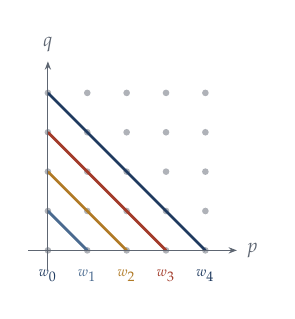
\begin{tikzpicture}[scale=0.5]
\foreach \p in {0,...,4} \foreach \q in {0,...,4} {\fill[Gris!50] (\p,\q) circle (2.4pt);}
\foreach \n/\c in {0/Bleu,1/BleuMoyen,2/Ocre,3/Brique,4/Bleu} {
  \draw[\c,line width=1pt] (\n,0) -- (0,\n);
  \node[font=\tiny\sffamily,\c,anchor=north] at (\n,-0.25) {$w_{\n}$};}
\draw[Gris,-{Stealth[length=3pt]}] (-0.5,0) -- (4.8,0) node[right,font=\scriptsize] {$p$};
\draw[Gris,-{Stealth[length=3pt]}] (0,-0.5) -- (0,4.8) node[above,font=\scriptsize] {$q$};
\end{tikzpicture}
\end{columns}
\pause
\begin{EX}
$\sum x^n$ par elle-même ($|x|<1$) : $w_n=(n+1)x^n$, donc $\sum(n+1)x^n=\frac1{(1-x)^2}$. Et $e^ae^b=e^{a+b}$ par le binôme.
\end{EX}
\end{frame}

% =====================================================================
\partie{1.6}{Synthèse}{Dans quel ordre poser les questions ?}{\rmI}

\begin{frame}{L'ordre des questions}
\centering
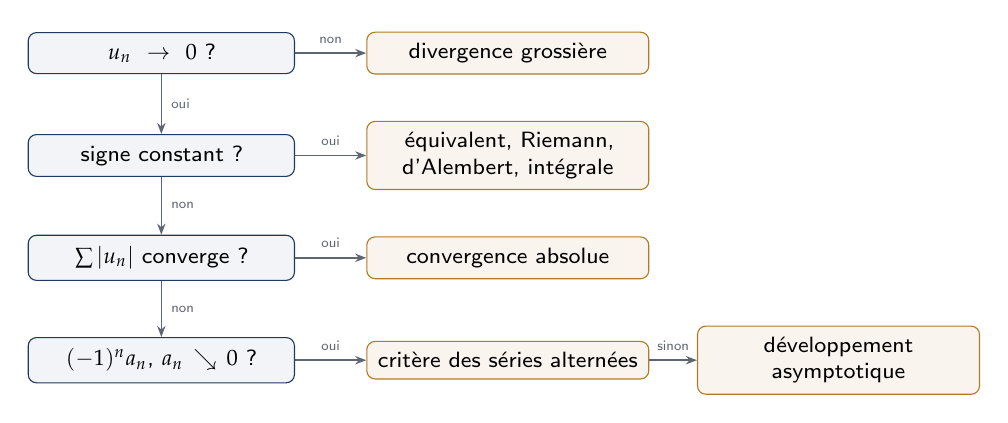
\begin{tikzpicture}[
  q/.style={draw=Bleu,fill=Fond,rounded corners=3pt,font=\footnotesize\sffamily,align=center,inner sep=4pt,text width=3.1cm},
  r/.style={draw=Ocre,fill=Ocre!8,rounded corners=3pt,font=\footnotesize\sffamily,align=center,inner sep=4pt,text width=3.3cm},
  f/.style={-{Stealth[length=4pt]},Gris,line width=0.6pt},l/.style={font=\tiny\sffamily,Gris}]
\node[q] (a) at (0,0) {$u_n\to0$ ?};
\node[r] (gr) at (4.4,0) {divergence grossière};
\node[q] (b) at (0,-1.3) {signe constant ?};
\node[r] (pos) at (4.4,-1.3) {équivalent, Riemann, d'Alembert, intégrale};
\node[q] (c) at (0,-2.6) {$\sum|u_n|$ converge ?};
\node[r] (acv) at (4.4,-2.6) {convergence absolue};
\node[q] (d) at (0,-3.9) {$(-1)^na_n$, $a_n\searrow0$ ?};
\node[r] (alt) at (4.4,-3.9) {critère des séries alternées};
\node[r] (dev) at (8.6,-3.9) {développement asymptotique};
\draw[f] (a) -- node[l,above]{non} (gr); \draw[f] (a) -- node[l,right]{oui} (b);
\draw[f] (b) -- node[l,above]{oui} (pos); \draw[f] (b) -- node[l,right]{non} (c);
\draw[f] (c) -- node[l,above]{oui} (acv); \draw[f] (c) -- node[l,right]{non} (d);
\draw[f] (d) -- node[l,above]{oui} (alt); \draw[f] (alt) -- node[l,above]{sinon} (dev);
\end{tikzpicture}
\end{frame}

\begin{frame}{\badgeexo{5}Synthèse}
\begin{ENONCE}[15 min]
Soit $u_0\in\,]-1,1[$, $u_{n+1}=\frac{1+u_n^2}2$ et $w_n=1-u_n$.
\begin{enumerate}
\item Montrer que $u_n\to1$ et que $w_{n+1}=w_n-\frac{w_n^2}2$.
\item En déduire que $\sum w_n^2$ converge.
\item Étudier $\sum\ln\frac{w_{n+1}}{w_n}$, puis $\sum w_n$.
\end{enumerate}
\objectif{séries télescopiques et équivalents dans un même raisonnement.}
\end{ENONCE}
\pause
\begin{INDICE}
(2) $w_n^2=2(w_n-w_{n+1})$. (3) $\ln\frac{w_{n+1}}{w_n}=\ln\left(1-\frac{w_n}2\right)$.
\end{INDICE}
\end{frame}

\begin{frame}{\badgecor{5}Synthèse}
\begin{columns}[T]
\column{0.36\textwidth}
\begin{RAIS}
Une suite et la série de ses différences ont même nature : on l'utilise dans les deux sens.
\end{RAIS}
\column{0.61\textwidth}
\etape{1.} $u_{n+1}-u_n=\frac{(1-u_n)^2}2\geq0$, majorée par $1$ : limite $\ell=\frac{1+\ell^2}2$, $\ell=1$.\\[3pt]
\pause
\etape{2.} $w_n^2=2(w_n-w_{n+1})$ : télescopique, $(w_n)$ converge : CV.\\[3pt]
\pause
\etape{3.} $\sum(\ln w_{n+1}-\ln w_n)$ : DV car $\ln w_n\to-\infty$. Or $\ln\left(1-\frac{w_n}2\right)\sim-\frac{w_n}2$, signe constant : $\sum w_n$ \textbf{DV}.
\end{columns}
\end{frame}

\begin{frame}{L'essentiel}
\begin{columns}[T]
\column{0.5\textwidth}
\begin{RETENIR}
\begin{itemize}
\item CV $\Rightarrow u_n\to0$ ; réciproque fausse.
\item Références : $\sum q^n$, $\sum\frac1{n^\alpha}$, $\sum\frac{x^n}{n!}$, télescopiques.
\item Termes positifs : comparaison, équivalents, d'Alembert, intégrale.
\end{itemize}
\end{RETENIR}
\column{0.46\textwidth}
\begin{RETENIR}
\begin{itemize}
\item Signe quelconque : absolue $\Rightarrow$ CV ; critère alterné ; développement.
\item Cauchy : séries absolument convergentes.
\end{itemize}
\end{RETENIR}
\end{columns}
\begin{PIEGE}
Équivalent sans signe constant ; d'Alembert avec $\ell=1$ ; $\sum_{n=0}^{+\infty}$ écrit trop tôt ; oublier la décroissance.
\end{PIEGE}
\end{frame}

\begin{frame}{Après la séance}
\begin{columns}[T]
\column{0.52\textwidth}
\begin{enumerate}
\item \textbf{Relire le livret} (chapitre~7) : démonstrations et exemples rédigés.
\item \textbf{Apprendre la fiche}.
\item Puis le \textbf{TD complet} (25 exercices, quatre parties).
\end{enumerate}
\column{0.42\textwidth}
\begin{ASTU}[Pour chercher seul]
Toujours dans le même ordre : $u_n\to0$ ? signe ? absolue ? alternée ? développement.
\end{ASTU}
\end{columns}
\end{frame}

\end{document}
